\section{Methodology}\label{sec:methodology}

\subsection{Problem Formulation}

Let $\mathcal{V} = \{1, \ldots, N\}$ denote $N{=}9$ administrative divisions. At forecast origin $t$, the model receives a lookback window of $T{=}7$ days and predicts targets at horizon $H{=}1$. Node features $\mathbf{X}^{\mathrm{node}} \in \mathbb{R}^{T \times N \times F_n}$ ($F_n{=}9$) encode division-level demand, supply, load, lags, rolling means, and regional shares. Global features $\mathbf{X}^{\mathrm{global}} \in \mathbb{R}^{T \times F_g}$ ($F_g{=}17$) encode calendar indicators, grid aggregates, limitation variables, and national generation scalars. Task~1 outputs regional demand $\hat{\mathbf{y}}^{\mathrm{demand}} \in \mathbb{R}^N$ (MW); Task~2 outputs graph-level OSI $\hat{y}^{\mathrm{osi}} \in [0,1]$.

OSI integrates three train-normalised components:
\begin{align}
c_1 &= L_{\mathrm{total}}/D_{\mathrm{total}}, \quad
c_2 = 1 - GR/\mathrm{Highest\_Gen}, \quad
c_3 = \mathrm{TOL}/\mathrm{Highest\_Gen}, \nonumber\\
\mathrm{OSI} &= \mathrm{mean}\bigl(\mathrm{minmax}_{\mathrm{train}}(c_1),\,
\mathrm{minmax}_{\mathrm{train}}(c_2),\,
\mathrm{minmax}_{\mathrm{train}}(c_3)\bigr),
\end{align}
where $L_{\mathrm{total}}$, $D_{\mathrm{total}}$, $GR$, and $\mathrm{TOL}$ denote total shedding, demand, generation reserve, and operational limitation. Same-day OSI is excluded from inputs when forecasting $\mathrm{OSI}(t{+}1)$ to prevent leakage.

The joint objective combines macro-averaged Huber loss on demand \cite{Huber1964RobustEstimation} with MSE on OSI:
\begin{equation}
\mathcal{L} = \mathcal{L}_{\mathrm{demand}}^{\mathrm{raw}}/100 + \lambda_2 \, \mathcal{L}_{\mathrm{osi}}, \quad \lambda_2 = 20.
\label{eq:loss}
\end{equation}
Demand-loss scaling prevents collapse to demand-only learning when OSI targets lie on $[0,1]$.

\subsection{Dataset and Graph Construction}

We use the Bangladesh Smart Grid dataset (Mendeley Data, Version~5) \cite{Hossain2025BangladeshSmartGrid}: 1,850 daily records (Nov.\ 2019--Dec.\ 2024) across nine divisions. Chronological partitions yield 1,281 training, 263 validation, and 264 test sliding windows (Table~\ref{tab:setup}). All preprocessing parameters---scaling, encoding, graph weights, OSI bounds---are estimated on training data only.

Pairwise Pearson correlations $\rho_{ij}$ on training-partition evening-peak demand define undirected edges with $\rho_{ij} \geq 0.65$; weights equal $\rho_{ij}$ and are row-normalised to form adjacency $\mathbf{A}$. This correlation-only graph (33 of 36 pairs retained) replaces geographical and hybrid priors following ablation evidence. Geographical adjacency (21 pairs) and hybrid adjacency (24 pairs) serve as ablation comparators only.

\subsection{PF-STGT Architecture}

Fig.~\ref{fig:1} shows the end-to-end pipeline; Fig.~\ref{fig:2} details configuration S2. Node and global tensors are embedded with regional identity and positional encoding. A \emph{spatial branch} applies graph-transformer self-attention over nodes at each timestep with additive bias from $\mathbf{A}$:
\begin{equation}
\mathrm{Attn}_{\mathrm{spatial}}(\mathbf{Q}, \mathbf{K}, \mathbf{V}) =
\mathrm{softmax}\!\left(\frac{\mathbf{Q}\mathbf{K}^\top}{\sqrt{d}} + \mathbf{B}_{\mathrm{adj}}\right)\mathbf{V}.
\label{eq:spatial}
\end{equation}
A \emph{temporal branch} applies a shared transformer encoder over each node's seven-day sequence. Learnable gating fuses the branches; the final timestep yields shared node embeddings $\mathbf{H}_{\mathrm{shared}}$. A per-node linear head decodes regional demand; a graph-level head combining pooled node states and global context decodes OSI through a bounded activation. Both tasks share encoders and differ only in decoding layers.

\begin{table}[htbp]
\caption{Dataset properties and frozen S2 training configuration}
\label{tab:setup}
\begin{center}
\scriptsize
\renewcommand{\arraystretch}{1.15}
\resizebox{\columnwidth}{!}{%
\begin{tabular}{|l|l|l|l|}
\hline
\textbf{Dataset} & \textbf{Value} & \textbf{Training} & \textbf{Value} \\
\hline
Divisions ($N$) & 9 & Optimiser & Adam, lr $5{\times}10^{-4}$ \\
Window ($T$) / horizon & 7 / 1 day & Batch / epochs & 32 / $\leq$200 \\
Node / global features & 9 / 17 & $\lambda_2$ (Eq.~\ref{eq:loss}) & 20.0 \\
Train / val / test windows & 1281 / 263 / 264 & Parameters & 749,058 \\
Graph edges ($\tau{=}0.65$) & 33 / 36 pairs & Early stop & Patience 15 \\
\hline
\end{tabular}%
}
\end{center}
\end{table}

\begin{figure}[!t]
\centering
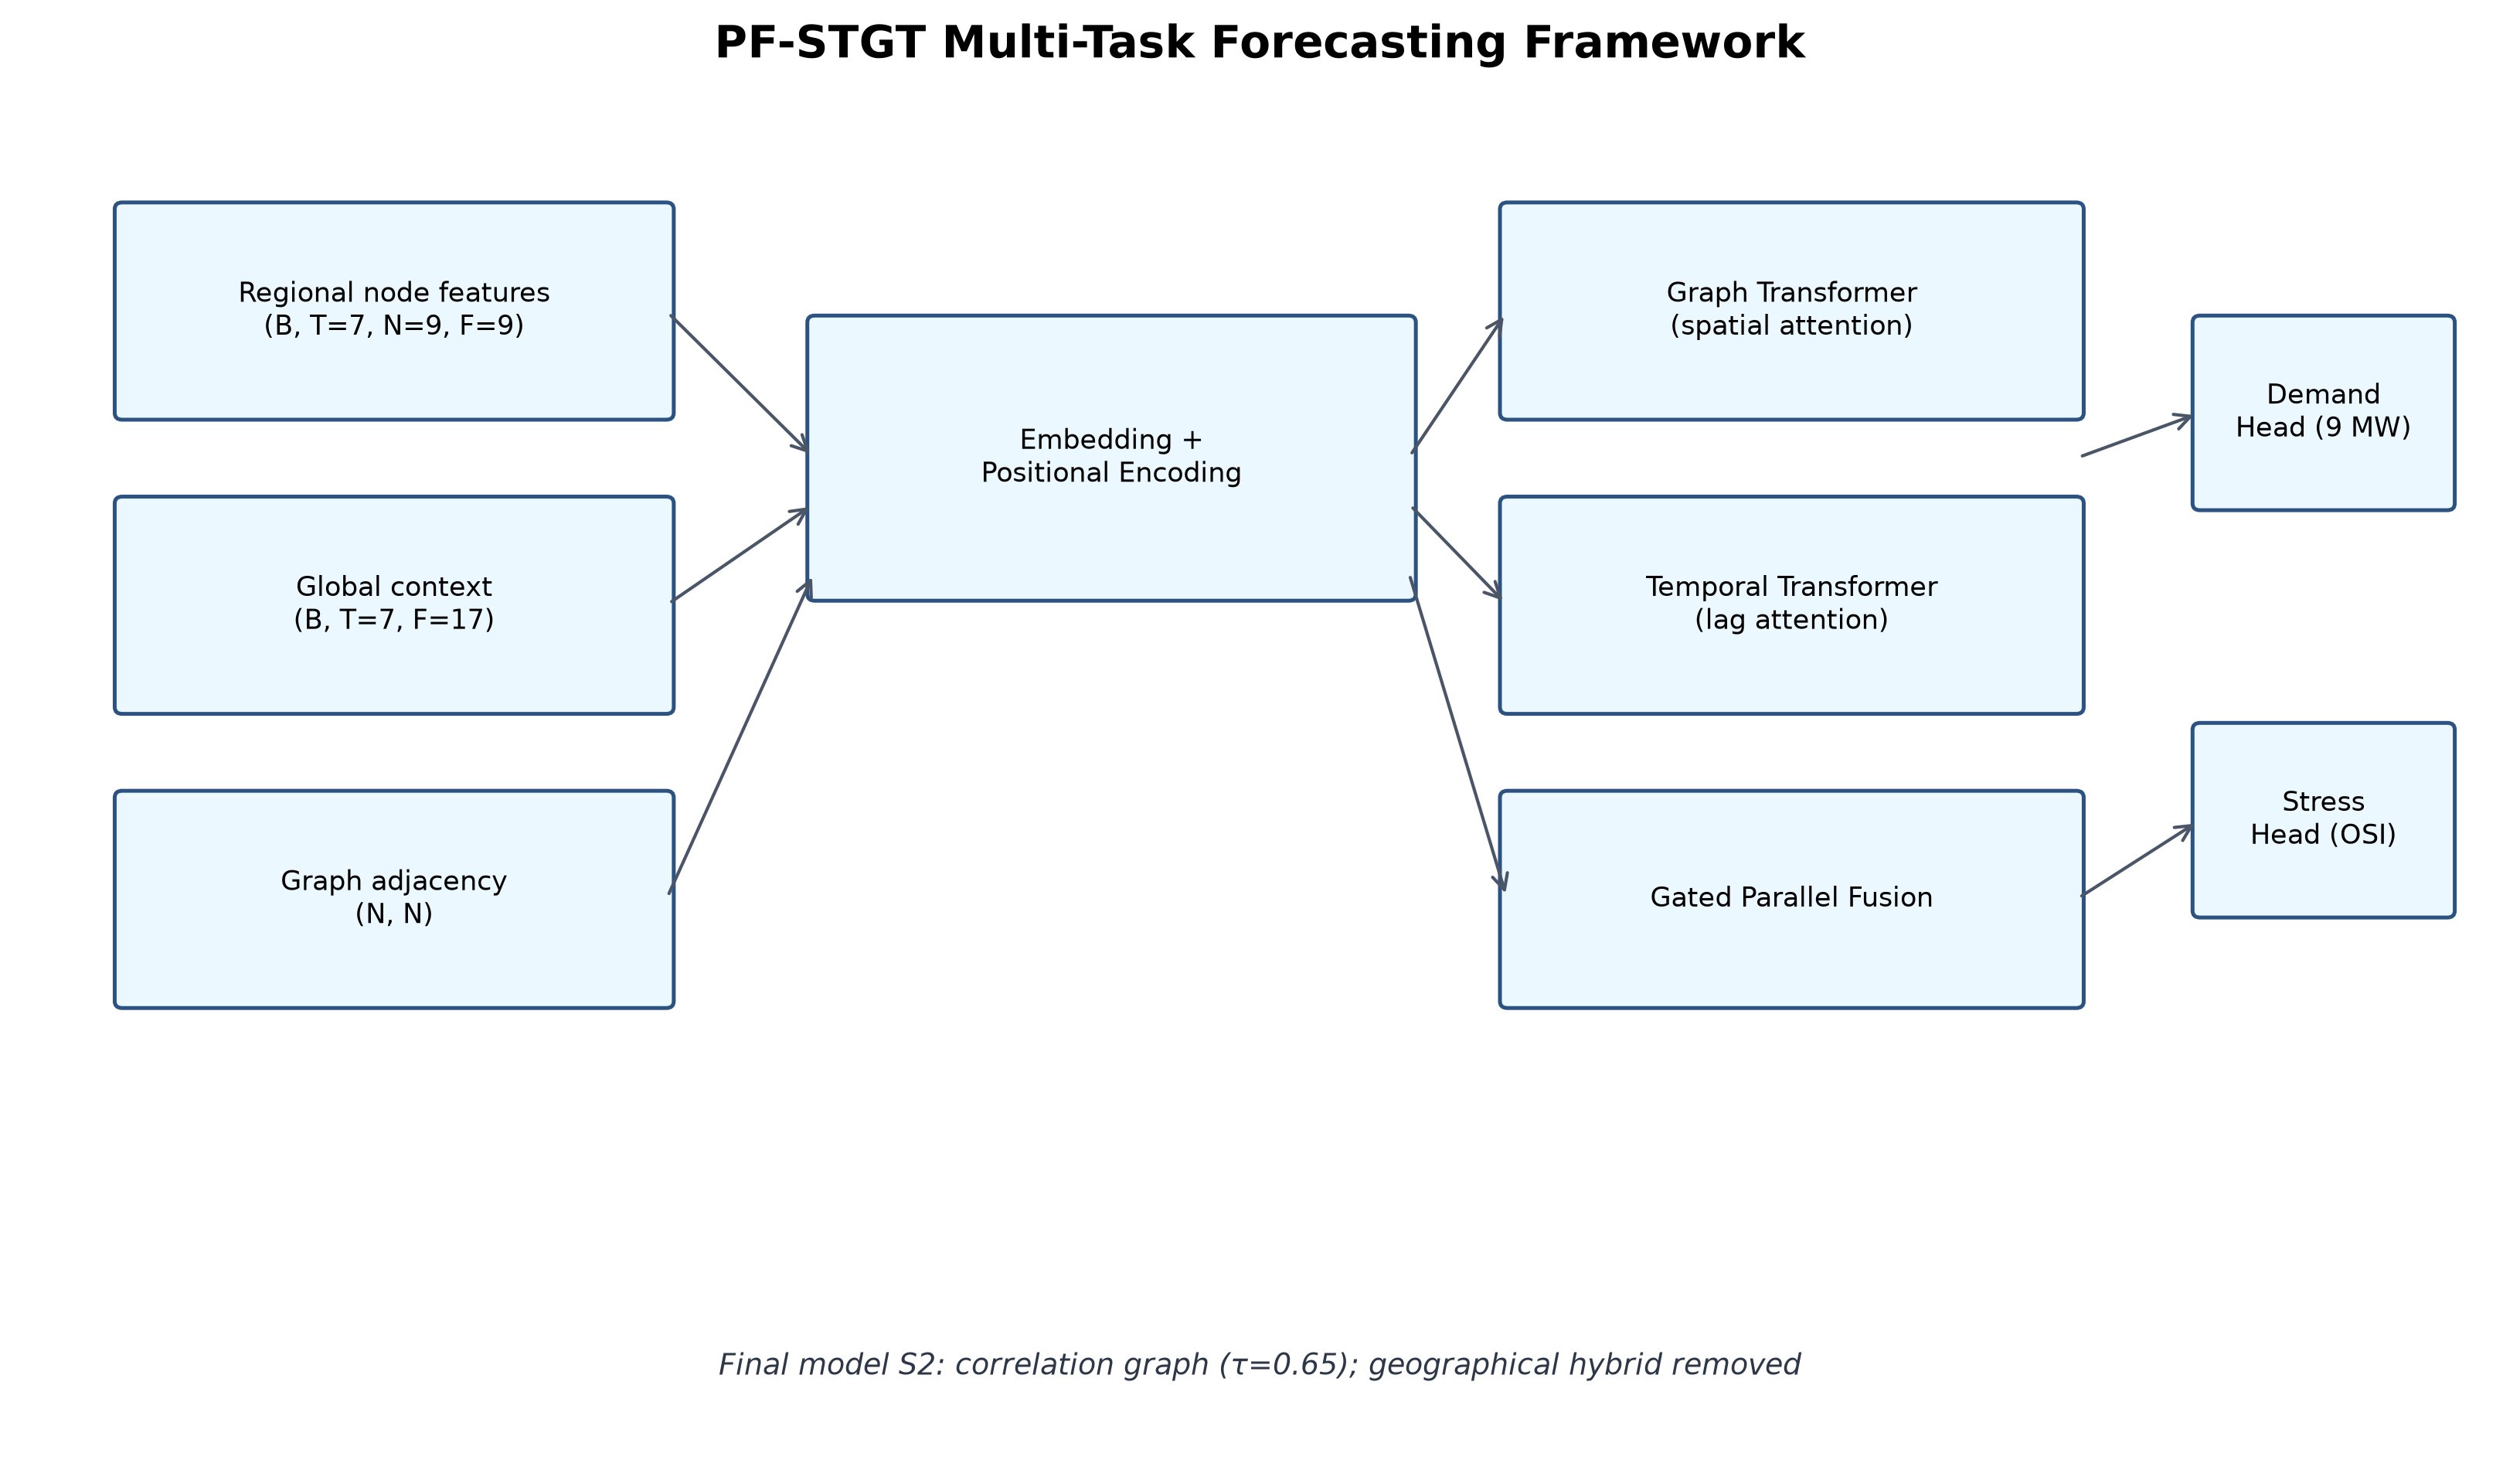
\includegraphics[width=\linewidth]{figures/figure_01_framework.png}
\caption{End-to-end PF-STGT multi-task forecasting framework.}
\label{fig:1}
\end{figure}

\begin{figure}[htbp]
\centering
% Shared IEEE publication figure palette (matches frozen asset specification)
\definecolor{ieeeblue}{HTML}{2c5282}
\definecolor{ieeelightblue}{HTML}{ebf8ff}
\definecolor{ieeegreen}{HTML}{276749}
\definecolor{ieeelightgreen}{HTML}{f0fff4}
\definecolor{ieered}{HTML}{c53030}
\definecolor{ieeelightred}{HTML}{fff5f5}
\definecolor{ieeegray}{HTML}{4a5568}
\definecolor{ieeedark}{HTML}{1a202c}
\definecolor{ieeeaccent}{HTML}{3182ce}
\definecolor{ieeemuted}{HTML}{718096}

\resizebox{\linewidth}{!}{%
\begin{tikzpicture}[
  font=\scriptsize,
  >=Stealth,
  s1box/.style={rectangle, draw=ieered, fill=ieeelightred, rounded corners=1.5pt,
    text width=3.6cm, minimum height=0.85cm, align=center, line width=0.45pt, inner sep=2pt},
  s2box/.style={rectangle, draw=ieeegreen, fill=ieeelightgreen, rounded corners=1.5pt,
    text width=3.6cm, minimum height=0.85cm, align=center, line width=0.45pt, inner sep=2pt},
  bluebox/.style={rectangle, draw=ieeeblue, fill=ieeelightblue, rounded corners=1.5pt,
    align=center, line width=0.45pt, inner sep=2pt},
  arr/.style={->, line width=0.55pt, color=ieeegreen}
]
% Title
\node[font=\small\bfseries, text=ieeedark] at (3.9,2.55)
  {S2 --- Correlation-Only PF-STGT (Final Architecture)};

% S1 -> S2 evolution
\node[s1box] (s1) at (0.9,1.75) {S1 (superseded)\\Hybrid geo + corr graph};
\node[s2box] (s2) at (6.9,1.75) {\textbf{S2 (final)}\\Correlation graph only};
\draw[arr] (s1.east) -- node[above, font=\fontsize{6}{7}\selectfont, text=ieeegreen] {$-$4.66 MW} (s2.west);

% Shared trunk
\node[bluebox, text width=7.8cm, minimum height=0.75cm] (trunk) at (3.9,0.75)
  {Shared trunk: PF-STGT --- Graph + Temporal transformers + Fusion (749{,}058 params)};

% Loss and metrics
\node[bluebox, text width=3.65cm, minimum height=0.8cm] (loss) at (1.95,-0.55)
  {Multi-task loss\\Huber$/100 + 20\cdot\mathrm{MSE}(\mathrm{OSI})$};
\node[bluebox, text width=3.65cm, minimum height=0.8cm] (met) at (5.85,-0.55)
  {Test demand MAE: 88.65 MW\\Stress $R^2$: 0.745};

% Connect trunk to bottom boxes
\draw[color=ieeegray, line width=0.35pt] (trunk.south) -- ++(0,-0.12) -| (loss.north);
\draw[color=ieeegray, line width=0.35pt] (trunk.south) -- ++(0,-0.12) -| (met.north);
\end{tikzpicture}%
}

\caption{Frozen S2 configuration: correlation-only graph PF-STGT with parallel-fusion encoding.}
\label{fig:2}
\end{figure}

